\documentclass[11pt]{article}

%%% Load some useful packages:
%% "New" LaTeX2e graphics support.
\usepackage{graphicx}
%%	using final option to force graphics to be included even in draft mode
%\usepackage[final]{graphicx}

%% Support sub-figures.
\usepackage{subfigure}

%% Make subsubsections numbered and included in ToC
\setcounter{secnumdepth}{3}
\setcounter{tocdepth}{3}

%% Package to linebreak URLs in a sane manner.
\usepackage{url}

%% Define a new 'smallurl' style for the package that will use a smaller font.
\makeatletter
\def\url@smallurlstyle{%
  \@ifundefined{selectfont}{\def\UrlFont{\sf}}{\def\UrlFont{\small\ttfamily}}}
\makeatother
%% Now actually use the newly defined style.
\urlstyle{smallurl}

%% Make margins less ridiculous
\usepackage{fullpage}

%% Allows insertion of fixme notes for future work
\usepackage[footnote, nomargin]{fixme}

%%%% Turned off for tech report, should be turned on for research portfolio
%% Turn on double spacing
%\usepackage{setspace}
%\doublespacing

%% Make URLs clickable
\usepackage[colorlinks, bookmarks=true]{hyperref}
\usepackage[all]{hypcap}


%% Since I'm using the LaTeX Makefile that uses dvips, I need this
%% package to make URLs break nicely
\usepackage{breakurl}

\usepackage{array}

%% Make table cross pages.
\usepackage{longtable}

\begin{document}

\title{Makahiki: A Serious Game Engine for Sustainability \\
\em  A Research White Paper}

\author{
	 Yongwen Xu \\
\em  Collaborative Software Development Laboratory \\
\em  Department of Information and Computer Sciences \\
\em  University of Hawai'i at Manoa\\
     yxu@hawaii.edu \\
}

\date{\today}
\maketitle

\tableofcontents

\graphicspath{{figures/}} 
\DeclareGraphicsExtensions{.eps} 

\newpage
\begin{abstract}

My research seeks to investigate how to build a customizable serious game engine for sustainability called Makahiki. It provides an open source, component-based, extensible framework for creating serious games for the purpose of education and behavioral change regarding energy, water, food, and waste generation and use. Different organizations configures the Makahiki framework to produce a ``challange instance'' with a specific set of game mechanics, user interface features, and experimental goals. Makahiki provides sophisticated instrumentation to support evaluation of how well the game mechanics supported the organization's goals for the challenge.

This white paper describes the Makahiki's research goal, system design, and experimental design on how to evaluate the effectiveness of the Makahiki as framework in developing serious games.
\end{abstract}


%% Contains introduction to the related work when used outside the
%% context of the dissertation proposal
\section{Introduction}

Sustainability education and conservation has become an international imperative due to the rising cost of energy, increasing scarcity of natural resources and irresponsible environmental practices. 
Over the past decade, running energy and water challenges have become a focal point for sustainability efforts at university, government, and industry campuses. Designers of those competitions have had three choices for information technology: (a) build their own custom in-house solution; (b) out-source to a commercial provider; or (c) use a "minimal tech" solution such as a web page and manual posting of data and results.

We developed a framework called Makahiki as a new choice: an extensible game engine for the development and evaluation of sustainability challenges. Makahiki has a unique feature set intended to foster more rapid innovation and development. These features include: (1) an open source license and development model which makes the technology available without charge and facilitates collaborative development and improvement; (2) support for an "ecosystem" of extensible, interrelated, customizable games and activities; (3) real-time game analytics and A/B testing for research and evaluation; (4) pedagogically organized and extensible learning activities; (5) a responsive user interface supporting mobile, tablet, and laptop displays; and (6) support for deployment to the cloud as an inexpensive option for hosting the competition.

The Makahiki framework will be used in 2012 by three organizations, namely, University of Hawaii at Manoa, Hawaii Pacific University, East West Center of University of Hawaii, to implement individually tailored sustainability challenges. 

\section{Research Goals}

There are two research goals in Makahiki: (a) provides an extensible framework to easily create engaging games for sustainability education and behavior change, and (b) provides an experimental test bed for Gamification research into the effectiveness of different game mechanics in the context of sustainability.

The challenges of creating a customizable game engine are:  (a) creating a new instance of Makahiki by selecting the games they want the system to support, and (b) extending Makahiki by writing new game components, and (c) supporting ease of use by non-technical organizations with minimal technical support.

In order to provide an experimental test bed for game research, Makahiki will be designed to support A-B testing, where different game mechanics could be configured using the game engine to create ``treatments'' for different user groups. The game engine will provide real-time game analytics to these treatments.

\section{System Design}

Makahiki consists of a configurable game engine that can be customized to the needs of
different organizations.  It includes a library of pre-built game ``widgets'' that
implement a variety of game mechanics.  Using the widgets, an organization can create a
custom energy challenge in which players can compete individually and/or in teams to earn
the most points by reducing their energy consumption as well as by learning about energy
concepts in general.

Figure \ref{fig:system-architecture} illustrates
the architecture of Makahiki.

\begin{figure}[htbp] %  figure placement: here, top, bottom, or page
   \centering
   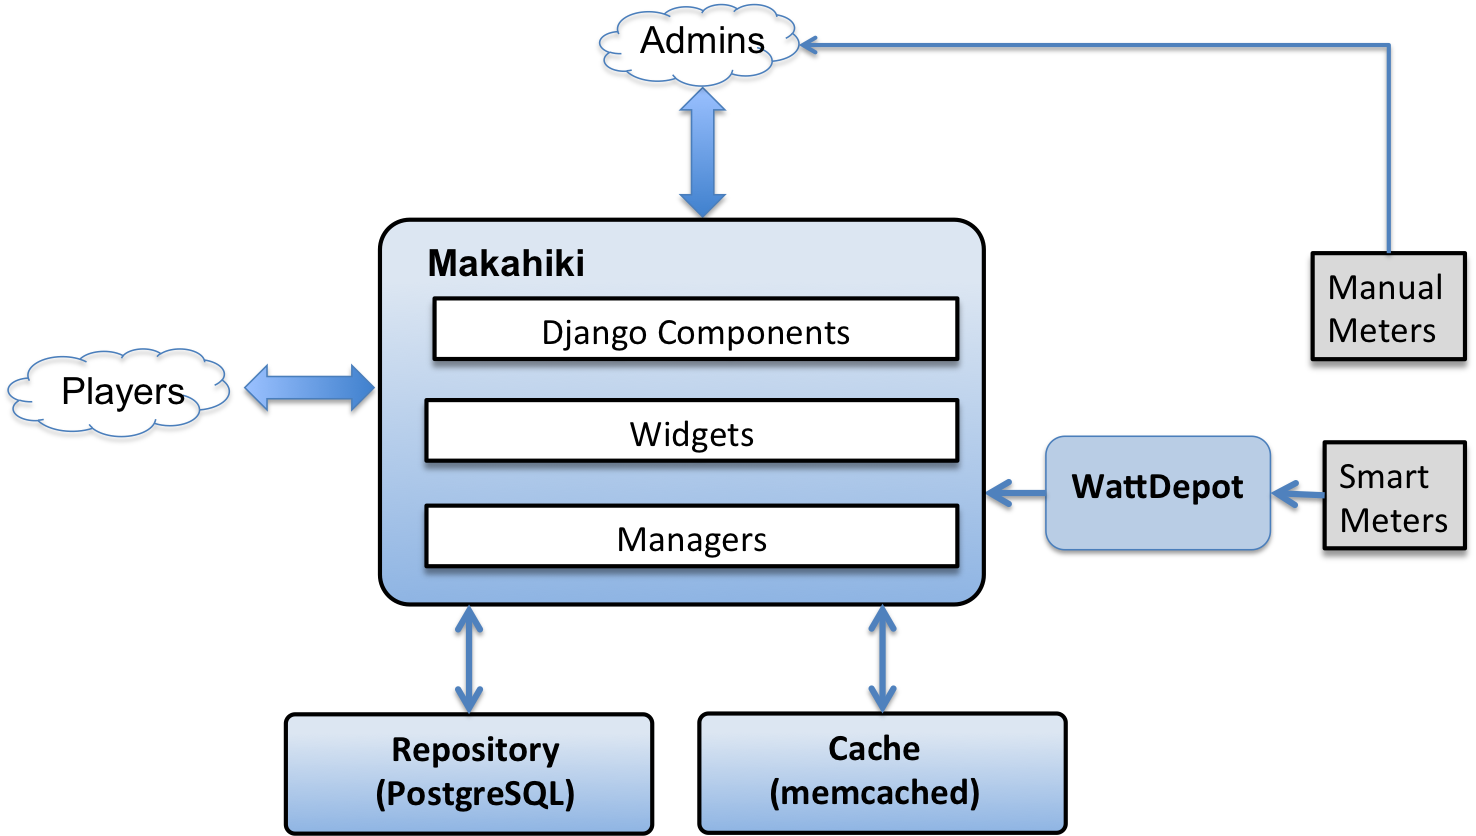
\includegraphics[height=20em]{system-architecture} 
   \caption{Makahiki System Architecture}
   \label{fig:system-architecture}
\end{figure}


\section{Experimental Design}

In order to evaluate how the Makahiki meets the research goals, we propose to investigate the following the research questions:

\begin{enumerate}

\em \item Can Makahiki be successfully deployed in multiple organizational scenarios to provide games for major sustainability issues (energy, water, waste, recycling, transportation, etc.)? \em
\em \item Can Makahiki provide an API and procedures to support enhancement with new features and capabilities with a minimum of impact on other aspects of the framework? \em
\em \item Can Makahiki provide an engaging and fun learning user interface to its end users? \em
\em \item Can Makahiki provide a mean to perform research on games for sustainability through A/B testing? \em

\end{enumerate}

\subsection{Site Admin Evaluation}
To evaluate question (1), we plan to perform the case study research on multiple case studies. It consists of surveys and interviews of administrators of all sites, asking for their assessment of the framework, whether it fulfilled their needs, and what they wish was different or better. 

\subsubsection{Methodology}

A \em post-challenge survey \em will be sent out to the administrators of three sites, namely, University of Hawaii at Manoa, Hawaii Pacific University, and East West Center at University of Hawaii, right after their challenges are completed. Before the Makahiki is used, the site admins are offered technical trainings about the use of Makahiki. We will record the training times, and interview the trainees about their feedback of the usability of the system. The effectiveness of the training will affect the result of the survey.

The survey contains ** questions and we expect that the time to complete is about 10 minutes. The completed questionnaire follows:

\begin{enumerate}

\item Install the Makahiki locally is: 
\begin{itemize}
\item don't need to install locally
\item Very Easy
\item Easy
\item Neither easy nor difficult
\item Difficult
\item Very Difficult
\end{itemize}

\item Installing the Makahiki in Heroku is: 
\begin{itemize}
\item don't need to install in Heroku
\item Very Easy
\item Easy
\item Neither easy nor difficult
\item Difficult
\item Very Difficult
\end{itemize}

\item Please describe any problem you encountered during the installation, either locally or in Heroku:

\item How long does it take you to complete the installation of Makahiki: 
\begin{itemize}
\item less than 10 minutes
\item about 1 hour
\item about 2 hour
\item more than 2 hours but less than a day
\item more than 1 day
\end{itemize}

\item Configuring the Makahiki to your organization's needs is: 
\begin{itemize}
\item Very Easy
\item Easy
\item Neither easy nor difficult
\item Difficult
\item Very Difficult
\end{itemize}

\item How long does it take you to complete the configuration of Makahiki to run your organization's challenge: 
\begin{itemize}
\item less than 1 hour
\item about 2 hour
\item more than 2 hours but less than a day
\item more than 1 day
\end{itemize}

\item Please describe the most difficult part(s) of the configuration you've encountered while configuring the Makahiki:

\item Administration using the Makahiki admin interface during the challenge is: 
\begin{itemize}
\item Very Easy
\item Easy
\item Neither easy nor difficult
\item Difficult
\item Very Difficult
\end{itemize}

\item How much time do you spend in administrating your organization's challenge using the Makahiki admin interface every day: 
\begin{itemize}
\item less than 10 minutes
\item about 1 hour
\item about 2 hours
\item about 4 hours
\item more than 4 hours
\end{itemize}

\end{enumerate}

\subsubsection{Data Collected}
\begin{itemize}
 \item time taken to install the Makahiki
 \item time taken to configure the Challenge
 \item number of problems encountered
 \item time taken in training
 \item number of problems encountered in training
 \item time taken in admining the challenge
 \item number of problems encountered during the admining the challenge
 
\end{itemize}

\subsection{Developer Evaluation Case Study}
To evaluate question (2), we plan to perform the case study research on at least one case. It consists of a ``case study'' of an external developer who is tasked with making an enhancement to the system.  Careful records of his interactions with developers, commits, and self-reported issues and problems along with interview data is used to determine how well the system achieved its goal as an extensible framework. The goal for the developer evaluation is to find out: (a) What kinds of learnings must occur, (b) What kind of background is necessary from a developer to enhance the system, (c) What kinds of problems were encountered and how they were resolved, (d) What kinds of changes to the system could be made to address the problems.

\subsubsection{Methodology}
\begin{enumerate}
\item \em Log Book\em: We will create a google Form for the developer to fill out at the end of each programming session. The content of the form follows:
 \begin{itemize} 
 \item Date and Time this session begins
 \item Length of the session (in minutes)
 \item Development activities (coding, documentation, debugging, testing, etc.)
 \item What was accomplished
 \item What problems occurred
 \item Please commit your code so that we have your latest changes.
 \end{itemize}

Figure \ref{fig:developer-eval-form} illustrates the google form used for Makahiki developer evaluation.

\begin{figure}[htbp] %  figure placement: here, top, bottom, or page
   \centering
   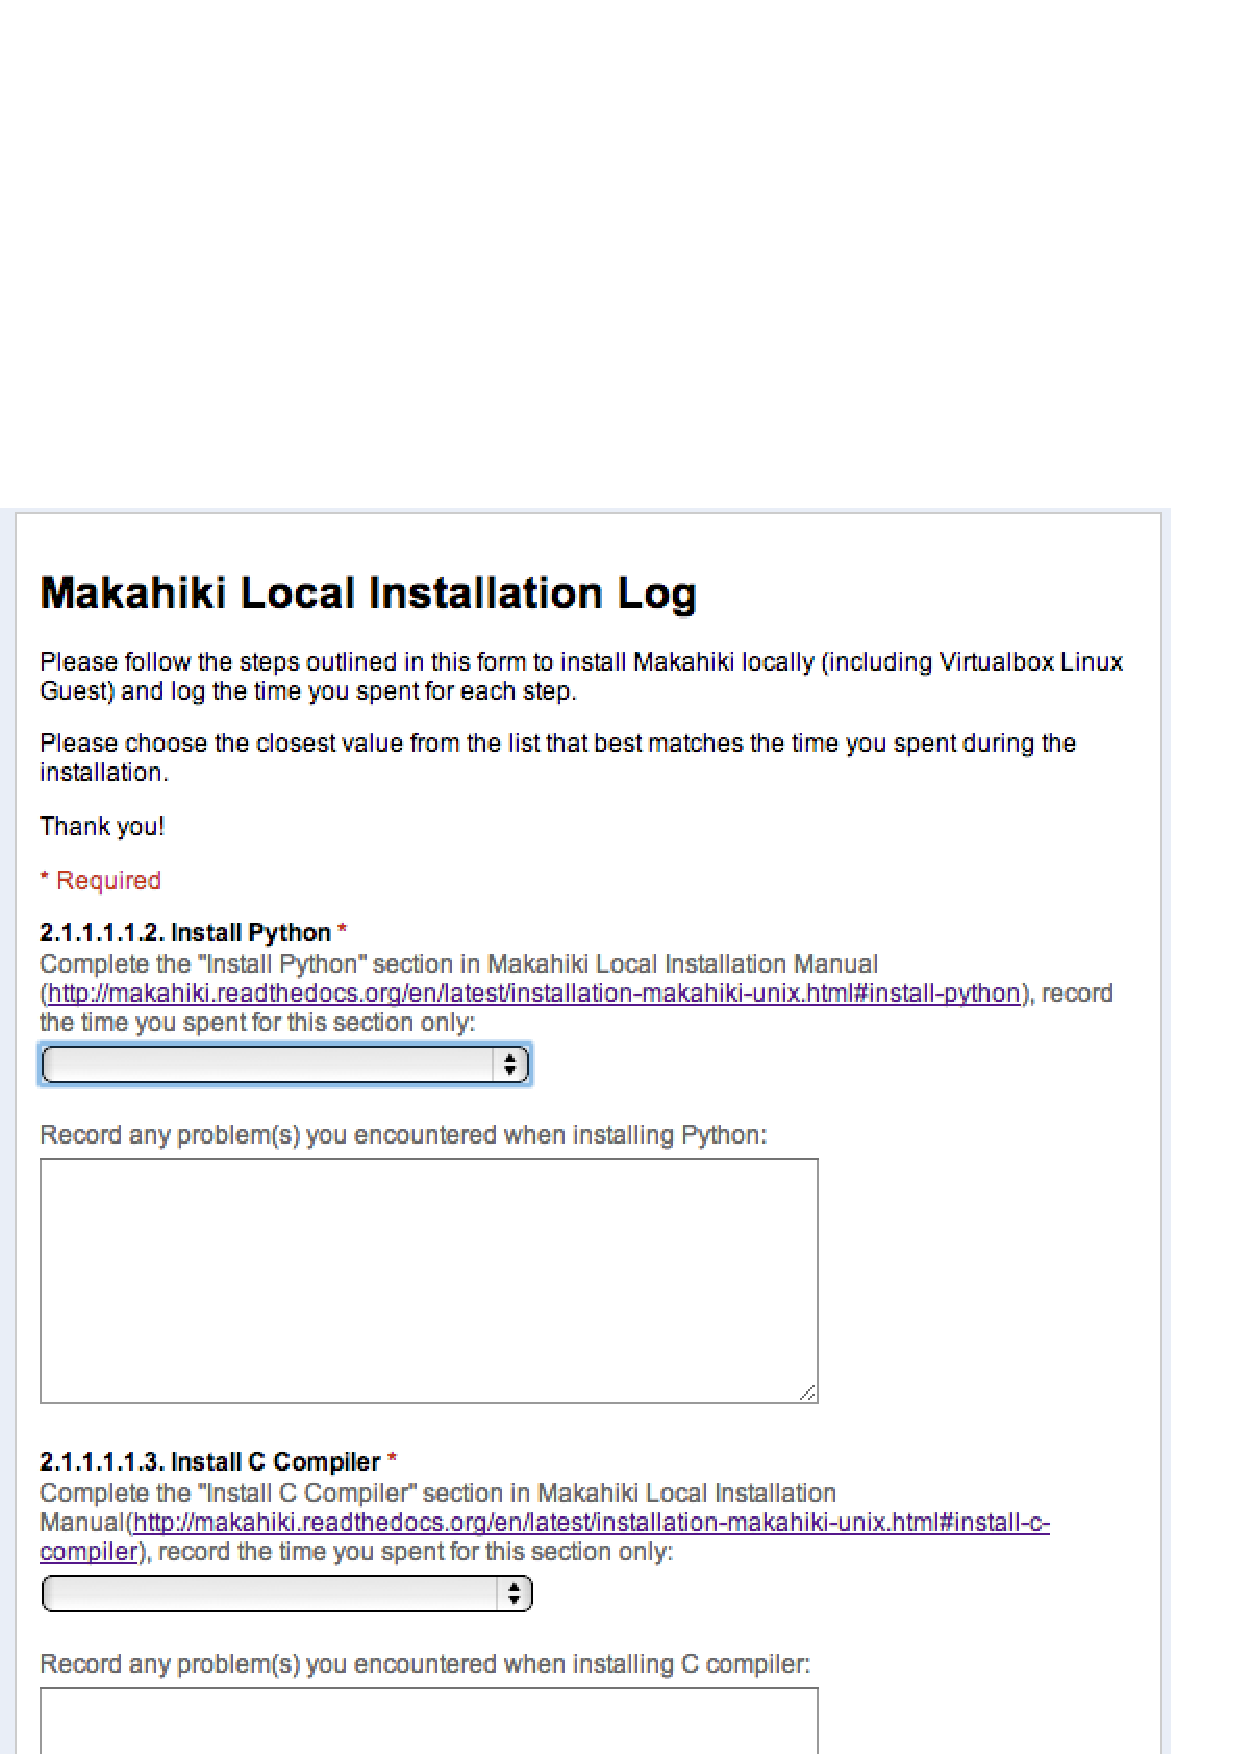
\includegraphics[height=25.5em]{developer-eval-form} 
   \caption{Makahiki Developer Evaluation Form}
   \label{fig:developer-eval-form}
\end{figure}
 
\item \em Meetings \em: We will have weekly developer meetings. we will record the meetings to support the analysis of development usability. we will focus on what kind of problems were encountered during the development.

\item \em Emails and Chat sessions \em: We will save the email exchanges with the developer and the online chat sessions for further analysis.

\end{enumerate}

\subsubsection{Data Collected}
\begin{itemize}
 \item time taken to setup the development env
 \item number of errors encountered
 \item interactions (emails, chats, meetings) with internal developers
 \item time spent in reading the doc initially
 \item time spent in reading the doc during the development
 \item time taken to create the initial revision of the enhancement
 \item time taken for unit testing, debugging
 \item time taken to integrate into the system
 \item number of makahiki APIs used
 \item metrics of commits, interactions in Github
 
\end{itemize}

\subsection{End User Evaluation}
To evaluate question (3), we plan to perform end users data collection and analysis using the framework itself. It consists of (a) in-game surveys of participants of all sites asking for their assessment of the game experience and its suitability to their situation;
(b) aggregated analytics data collected from all sites, providing insight into what parts of site were used in what ways.

\subsubsection{Methodology}

\em In-game surveys \em will be implemented as activities in smartgrid game in the challenge. We plan to have one in-game survey for each round. Players can earn points by completing the survey.

Each survey consists of ** questions and expected to be completed within 5 minutes. The questionares of the survey follows:

\begin{enumerate}

\item How would you feel about the user interface of the Kukui Cup? 
\begin{itemize}
\item Hard to use
\item Boring
\item confusing
\item so so
\item fun
\item additive
\end{itemize}

\item How much time you use Kukui Cup via mobile devices (phones and tablets) v.s computer?
\begin {itemize}
\item mobile device only
\item mostly mobile device
\item half mobile device and half computer
\item mostly computer
\item computer only
\end{itemize}

\item Do you find the Kukui Cup application responsive? In other worlds, did web pages load quickly and correctly?
\begin {itemize}
\item quick and responsive
\item it is fine
\item a little bit slow
\item slow
\item very slow and problematic
\end{itemize}

\item When you logged in for the first time, you are prompted with a series of screens to set up your profile. How do you feel about this "first login sequence"?
\begin{itemize}
\item easy to follow
\item hard to follow
\item too many steps
\item no problem at all
\item others (please specify)
\end{itemize}

\item After finishing the first login sequence, the application took you to the home page.  Were you confused at that point about what to do next? 

\item Did you try accessing the application from a smart phone?  If so, please tell us what kind of phone you used and whether or not you encountered any problems

\item Did you think the "Quests" are helpful in learning how to play the game? What do you think we could do to make it easier to learn to play the game?

\item  Did you have any problems using the smart grid game?  Was it easy to understand how to unlock new levels? 

\item Did you think the "Badges" are helpful in motivating you to play the game more? 
\begin{itemize}
\item Yes, specify what do you like about the badges.
\item No, specify what do you not like about the badges
\end{itemize}

\item Was it easy to understand how to play the Raffle game? Did you encounter any difficulties playing the game?

\item Did you encounter any problem using your mobile device to use the Kukui Cup? If so, what problem did you encounter?

\item What game(s), or page(s) in the kukui cup application did you like the most?

\item What would you consider to be the single most important thing for us to improve in the application?

\end{enumerate}

Besides in-game surveys, we plan to collect the data displayed in the Makahhiki's real-time analytics page. The analytics we are interested in for evaluating usability are:

\begin{itemize}
 \item Popular Quests, Events, Activities, Commitments, RSVPs
 \item Referrals
 \item Daily logins, New Users
 \item Action Feedback
\end{itemize}

\subsection{A/B Testing Evaluation Case Study}
To evaluate question (4), we plan to perform the case study research on at least one case. It consists of a ``case study" of one A/B test from three sites in order to answer the following research question: What level of energy data "latency" is required to provide useful feedback to participants in energy challenges like the Kukui Cup?  To assess this, we will implement three levels of energy latency:  (a) Subminute-level latency through the Power Meter at Hawaii Pacific University site; (b) Hour-level latency through the Daily Energy Goal Game at University of Hawaii site (no Power Meter); and (c) Day-level latency through the manual Daily Energy Goal Game at East West Center site.  In-game surveys will  be used at each site to determine how much participants interacted with the given type of feedback, and whether they felt limited by the given level of latency.

\subsubsection{Methodology}

\subsubsection{Data Collected}
  
%% Use this for an alphabetically organized bibliography
%%\bibliography{sustainability,csdl-trs,gamification}
%%\bibliographystyle{plain}

\end{document}
